\documentclass[11pt,a4paper]{article}

\usepackage[T1]{fontenc}
\usepackage[utf8]{inputenc}
\usepackage{lmodern}
\usepackage{microtype}
\usepackage{amsmath,amssymb,amsthm,mathtools,bm}
\usepackage{booktabs,array,tabularx,longtable}
\usepackage{graphicx,float,caption}
\usepackage{xcolor}
\usepackage[margin=23mm]{geometry}
\usepackage{enumitem}
\usepackage{fancyhdr}
\usepackage{hyperref}

\definecolor{finblue}{HTML}{1F5A99}
\definecolor{finorange}{HTML}{C45A00}
\definecolor{fingreen}{HTML}{19733A}
\definecolor{finred}{HTML}{A61B1B}
\definecolor{finpurple}{HTML}{6B3FA0}
\definecolor{finsoft}{HTML}{F2F5F8}
\definecolor{fingray}{HTML}{4E5964}

\hypersetup{
  colorlinks=true,
  linkcolor=finblue,
  citecolor=fingreen,
  urlcolor=finblue,
  pdftitle={FIN Programs P507-P516: Nonlinear Source and Certified Localization},
  pdfauthor={Krzysztof Żuchowski},
  pdfsubject={Quartic-source obstruction, parametric Krawczyk continuation, orbital stability, memory robustness, transcendental clock ratio, and robust observability},
  pdfkeywords={FIN, DNLS, nonlinear source, Krawczyk, orbital stability, Stieltjes memory, Lindemann-Weierstrass, PSD, identifiability}
}

\pagestyle{fancy}
\fancyhf{}
\fancyhead[L]{\small FIN Programs P507--P516}
\fancyhead[R]{\small Release 10.51}
\fancyfoot[C]{\thepage}
\setlength{\headheight}{14pt}

\newtheorem{theorem}{Theorem}[section]
\newtheorem{proposition}[theorem]{Proposition}
\newtheorem{corollary}[theorem]{Corollary}
\theoremstyle{definition}
\newtheorem{definition}[theorem]{Definition}
\theoremstyle{remark}
\newtheorem{remark}[theorem]{Remark}

\newcommand{\C}{\mathbb C}
\newcommand{\R}{\mathbb R}
\newcommand{\Z}{\mathbb Z}
\newcommand{\status}[2]{\textcolor{#1}{\textbf{[#2]}}}
\newcommand{\proven}{\status{fingreen}{PROVEN}}
\newcommand{\strong}{\status{finblue}{STRONG EVIDENCE}}
\newcommand{\moderate}{\status{finorange}{MODERATE EVIDENCE}}
\newcommand{\refuted}{\status{finred}{REFUTED}}
\newcommand{\conditional}{\status{fingray}{CONDITIONAL}}
\newcommand{\claimbox}[1]{\begin{center}\fcolorbox{finblue}{finsoft}{\parbox{0.91\textwidth}{#1}}\end{center}}

\setlist[itemize]{leftmargin=*,topsep=3pt,itemsep=2pt}
\setlist[enumerate]{leftmargin=*,topsep=3pt,itemsep=2pt}
\setlength{\emergencystretch}{2em}

\begin{document}
\hypersetup{pageanchor=false}

\begin{titlepage}
\centering
\vspace*{15mm}
{\Huge\bfseries FIN Programs P507--P516\par}
\vspace{5mm}
{\Large Nonlinear Source Obstruction and\par}
{\Large Certified Localization\par}
\vspace{4mm}
{\large Stability, memory, arithmetic, passivity, and law identifiability\par}
\vspace{15mm}
{\Large Krzysztof Żuchowski\par}
\vspace{2mm}
{\normalsize Independent Researcher --- Fractal Information Theory Project\par}
{\normalsize ORCID: 0009-0002-0909-3613\par}
\vspace{10mm}
{\large FIN Release 10.51 --- Version 1.0.0\par}
{\large 10 August 2026\par}
\vfill
\begin{minipage}{0.90\textwidth}
\small
\textbf{Scope.} This report executes P507--P516, the ten bounded continuations recommended after P497--P506. It asks whether the localized strict-DNLS state can be certified and whether its focusing law follows from FIN.

\medskip
\textbf{Evidence boundary.} Exact finite arguments, transcendence theory, outward interval arithmetic, finite-matrix spectral calculations and synthetic operational models are admitted. No laboratory record, external audit, dimensional calibration or physical-particle identification is asserted.

\medskip
\textbf{Runtime.} The complete deterministic research batch ran locally in approximately 57 seconds. Eleven regression and certificate tests passed.

\medskip
\textbf{Repository.} \url{https://github.com/hyconiek/Fractal-Nadsoliton-Theory}

\textbf{License.} CC BY 4.0.
\end{minipage}
\vfill
\end{titlepage}
\hypersetup{pageanchor=true}

\begin{abstract}
Ten follow-up studies are completed. They produce one decisive negative theorem and two substantial positive theorems.

First, the strict quadratic action cannot determine the focusing cubic term used in P497. The family
\[
 E_{\sigma,g}(\psi)=\frac12\langle\psi,A\psi\rangle+\frac{\sigma g}{4}\sum_x|\psi_x|^4,
 \qquad \sigma\in\{-1,+1\},\ g>0,
\]
has the same value, gradient and Hessian through second order at the zero state for both signs and every $g$, but produces opposite cubic Hamiltonian terms. Hence no observation confined to the strict quadratic or linear core can select focusing, defocusing, or the nonlinear coefficient. P497 therefore requires a quartic source functional, nonlinear datum, or an explicit axiom.

Second, the complete localized P497 branch is upgraded from numerical continuation to a parametric Krawczyk certificate. Four hundred and one uniform charts cover $0\le\kappa\le1$; every chart has strict Krawczyk inclusion and Jacobian defect below $0.006276$. Four hundred point certificates are nested in adjacent chart pairs and identify the same root across every interface. This proves one connected, fold-free real stationary branch throughout the declared strict-DNLS coupling interval. The result is conditional on the supplied focusing law.

Third, the ratio of the first two nonzero strict frequencies is proved transcendental. Since $\phi=650/4000$ and $\omega=743/4000$, every kernel phase is an integer multiple of $1/4000$. With $z=e^{i/4000}$, each Fourier eigenvalue is a Laurent polynomial in the transcendental number $z$ with algebraic coefficients. The mode-one polynomial has a nonzero highest $d=6$ term absent from mode two, so the polynomials are not proportional. An algebraic ratio would make $z$ algebraic, contradicting Lindemann--Weierstrass.

At $\omega=1$, the finite-DNLS GSS/Vakhitov--Kolokolov sign ledger has a simple phase kernel, one negative $L_+$ direction, positive spectral margins above one, and $dP/d\omega=0.617852>0$. The slope changes sign at $\omega\approx0.722143689$, so the wider frequency tube contains two stability sectors. The standard equal-power site/bond Peierls--Nabarro comparison is refuted for the P497 state because the localized bond branch has minimum power $4.06764$, above the site power $2.88168$, before it delocalizes.

Localization survives a declared positive Stieltjes--Bernstein memory loading, ending at IPR $0.620802$. A Wiener--resolvent analysis proves the $n^{-0.8}$ context-error rate class but yields a usable normalized bound only from $C_{1536}$ onward. An outward interval phase diagram proves non-PSD for $t<0.7008185567101464$, PSD for $t>0.7008185570593923$, and confines the only transition to the intervening width-$3.49\times10^{-10}$ bracket. The one-context synthetic tester remains separated under explicit preparation, measurement and timing budgets with worst-case TV margin $0.202414$. Finally, finite-dimensional polynomial parameter laws attain the dimension-minimal observation count only after the law class is supplied.

The branch is therefore mathematically real and now certified inside the added DNLS model, while its nonlinear source remains absent from FIN. This is progress and an obstruction, not a completed physical theory.
\end{abstract}

\noindent\textbf{Status vocabulary.}
\proven{} denotes an analytic theorem or outward finite certificate in its declared model;
\strong{} denotes robust finite numerical evidence;
\conditional{} marks dependence on an added law or operational budget;
\moderate{} denotes a bounded but incomplete result;
\refuted{} denotes failure of a precisely stated proposal.

\tableofcontents
\newpage

\section{Executive results}

\claimbox{\textbf{Central conclusion.} The localized strict-DNLS branch is no longer merely a numerical observation: P508 certifies it across the complete coupling interval. However, P507 proves that the present strict quadratic core cannot choose the focusing nonlinearity that creates the branch. The mathematical localization theorem is therefore genuine but explicitly axiom-augmented.}

\begin{longtable}{@{}p{0.07\textwidth}p{0.24\textwidth}p{0.39\textwidth}p{0.22\textwidth}@{}}
\caption{Programs, new objects, and terminal verdicts.}\\
\toprule
ID & New typed object & Main result & Status\\
\midrule
\endfirsthead
\toprule
ID & New typed object & Main result & Status\\
\midrule
\endhead
P507 & O211 quartic-jet source obstruction & The quadratic strict core cannot select cubic sign or strength. & \proven\\
P508 & O212 parametric Krawczyk tube & 401 charts plus 400 nested interfaces certify one fold-free branch on $[0,1]$. & \proven{} / \conditional\\
P509 & O213 orbital-stability ledger & GSS/VK signs hold at $\omega=1$; a slope transition occurs near $0.72214$. & \strong{} / \conditional\\
P510 & O214 equal-power PN existence audit & The localized bond branch never reaches the P497 site power. Standard PN comparison is unavailable. & \refuted\\
P511 & O215 memory-loaded branch & Localization survives the declared full positive Stieltjes memory loading. & \strong{} / \conditional\\
P512 & O216 frequency-ratio certificate & $\lambda_2/\lambda_1$ is transcendental and therefore irrational. & \proven\\
P513 & O217 Wiener--resolvent envelope & Rate class certified; normalized bound is too loose below $C_{1536}$. & \proven{} / \moderate\\
P514 & O218 global PSD phase diagram & Complete interval classification outside one width-$3.49\times10^{-10}$ root bracket. & \proven\\
P515 & O219 robust tester budget & Declared one-context separation retains worst-case TV margin $0.202414$. & \conditional\\
P516 & O220 polynomial-law design & Dimension-minimal observations work only after a finite law class is supplied. & \conditional{} / \proven\\
\bottomrule
\end{longtable}

\section{Shared objects and noninheritance rule}

The strict generator remains
\[
 W_{xy}=\frac{\cos(0.18575d(x,y)+0.16250)}{1+d(x,y)^{9/5}},
 \qquad A=\operatorname{diag}(W\mathbf1)-W\succeq0
\]
on $\Z/12\Z$. The localized branch uses the added focusing equation
\begin{equation}
 i\dot\psi=\kappa A\psi-|\psi|^2\psi,
 \qquad
 \kappa Au+\omega u-u^{\circ3}=0.
 \label{eq:dnls}
\end{equation}
Nothing in this report silently identifies the strict kernel with the legacy ontological kernel or transfers legacy electromagnetic, hierarchy, Planck-scale, matter, or gravity roles.

\section{P507 --- the nonlinear-source obstruction}

Use the convention $i\dot\psi=2\partial E/\partial\overline\psi$ and define
\[
 E_{\sigma,g}(\psi)=\frac12\langle\psi,A\psi\rangle
 +\frac{\sigma g}{4}\sum_x|\psi_x|^4.
\]

\begin{theorem}[Quadratic-core insufficiency]
For every $g>0$, the two functionals $E_{-1,g}$ and $E_{+1,g}$ have identical value, first derivative and Hessian at $\psi=0$, while their Hamiltonian flows contain opposite cubic terms. Moreover, changing $g$ leaves all quadratic/linear strict records invariant.
\end{theorem}
\begin{proof}
The difference is $(g/2)\sum_x|\psi_x|^4$, whose derivatives of order zero, one and two vanish at the origin. The Hamiltonian derivative of the quartic term is $\sigma g|\psi_x|^2\psi_x$. Thus the sign and $g$ live in the fourth-order jet and cannot be reconstructed from the common second-order jet $A$.
\end{proof}

At the anti-continuum limit with $\omega=1$, a nonzero one-site state satisfies
\[
 \omega u+\sigma g u^3=0,\qquad u^2=-\frac{\omega}{\sigma g}.
\]
It is real for focusing $\sigma=-1$ and impossible for defocusing $\sigma=+1$ at the same positive $\omega$. The scaling $u_g=u_1/\sqrt g$ also shows that normalized shape and IPR cannot identify $g$.

\paragraph{Verdict.} P507 does not find the missing source; it proves where it must enter. A quartic information/variational functional, a nonlinear response datum, or a focusing axiom is necessary. The current strict quadratic core alone cannot generate P497.

\section{P508 --- complete Krawczyk certification}

Let
\[
 F(u,\kappa)=\kappa Au+u-u^{\circ3}.
\]
For a box $X$ around a numerical centre $x_0$, parameter interval $K$ and approximate inverse $R\approx D_uF(x_0,\kappa_0)^{-1}$, the parametric Krawczyk image is
\[
 \mathcal K(X,K)=x_0-RF(x_0,K)
 +\bigl(I-RD_uF(X,K)\bigr)(X-x_0).
\]
Strict inclusion $\mathcal K(X,K)\subset\operatorname{int}X$ proves a unique zero in $X$ for every $\kappa\in K$ when the corresponding defect norm is below one.

The strict entries of $A$ were first enclosed with 70-decimal interval evaluation and then propagated with outward binary64 endpoints. The complete certificate has:
\begin{itemize}
\item 401 parameter charts covering $[0,1]$;
\item zero failed charts;
\item maximum state-box radius $1.4008843\times10^{-3}$;
\item maximum $\|I-RD_uF\|_\infty$ bound $0.00627510$;
\item minimum strict inclusion margin $1.33189\times10^{-7}$;
\item 400 point Krawczyk boxes at chart interfaces, each nested in both adjacent state boxes.
\end{itemize}

\begin{theorem}[Certified complete localized branch]
In the supplied focusing DNLS with the declared strict decimal operator, the one-site anti-continuum branch extends as one unique real, nonsingular and fold-free stationary branch for every $0\le\kappa\le1$.
\end{theorem}
\begin{proof}
Parametric Krawczyk inclusion proves one unique root in every chart for each parameter in its interval and nonsingularity of every stationary Jacobian there. At every adjacent chart interface, a point certificate nested in both boxes supplies a common exact root. Uniqueness identifies the roots, so the charts glue to one branch over the complete interval.
\end{proof}

\begin{figure}[H]
\centering
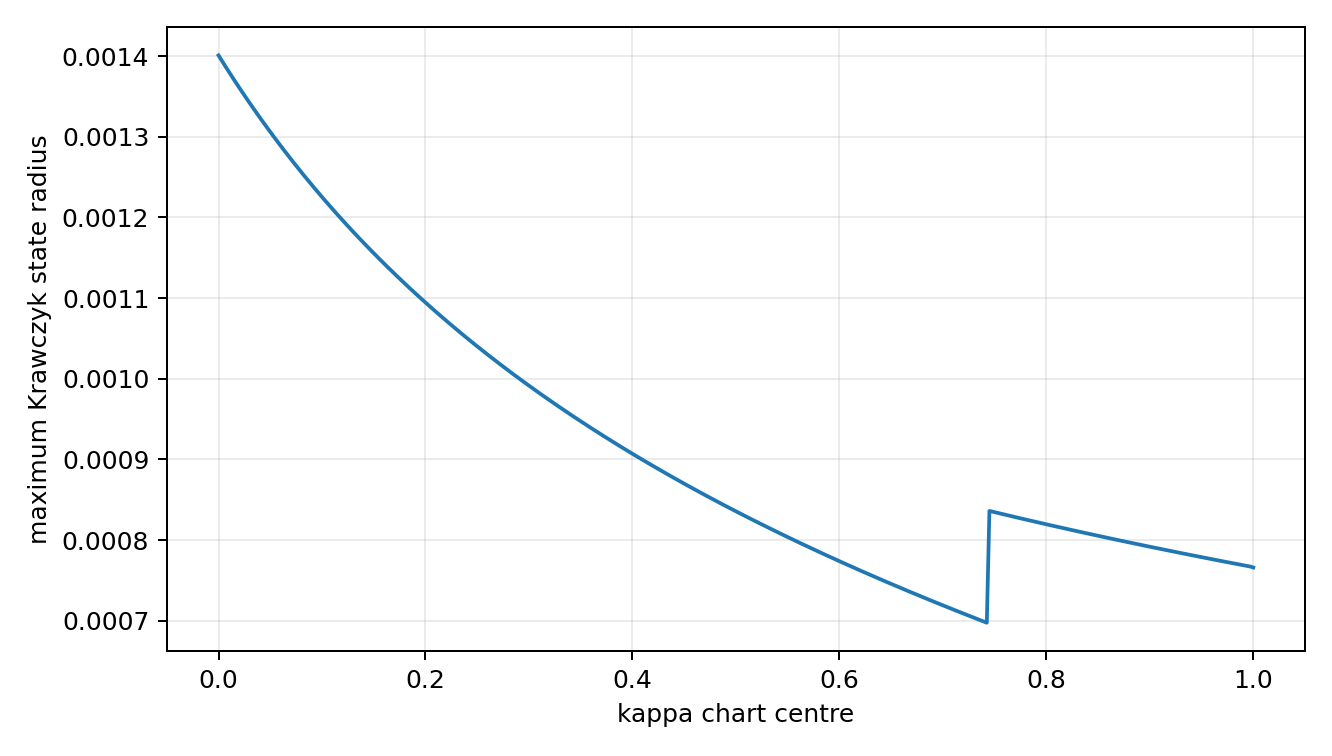
\includegraphics[width=0.77\textwidth]{FIN_Programs_507_516_Figures/p508_krawczyk_tube.png}
\caption{Maximum state radius of the 401 accepted parametric Krawczyk charts. The change near $\kappa\approx0.75$ reflects the adaptive interval geometry, not a branch discontinuity.}
\end{figure}

This theorem is stronger than P497's local IFT plus floating continuation. It remains conditional on the focusing law, $\omega=1$, the finite $\Z_{12}$ carrier and the declared strict decimal parameters.

\section{P509 --- orbital-stability sign structure}

For a standing wave at full coupling define
\[
 L_- = A+\omega I-\operatorname{diag}(u^2),\qquad
 L_+ = A+\omega I-3\operatorname{diag}(u^2).
\]
At $\omega=1$:
\begin{align*}
 \|L_-u\|&=2.94\times10^{-16}, &
 \lambda_2(L_-)&=1.23227663,\\
 n_-(L_+)&=1, &
 \lambda_2(L_+)&=1.04129123,\\
 \frac{dP}{d\omega}&=-2u^TL_+^{-1}u=0.61785192.&
\end{align*}
Thus the standard finite-DNLS GSS/Vakhitov--Kolokolov hypotheses are strongly satisfied numerically at the P497 point. They imply orbital stability modulo global phase after the usual finite Hamiltonian theorem is admitted.

The wider $0.6\le\omega\le1.4$ tube is not uniform. Its power slope vanishes at
\[
 \omega_{\rm VK}=0.7221436888572245\ldots
\]
and becomes negative below it while the inertia signs remain unchanged.

\begin{figure}[H]
\centering
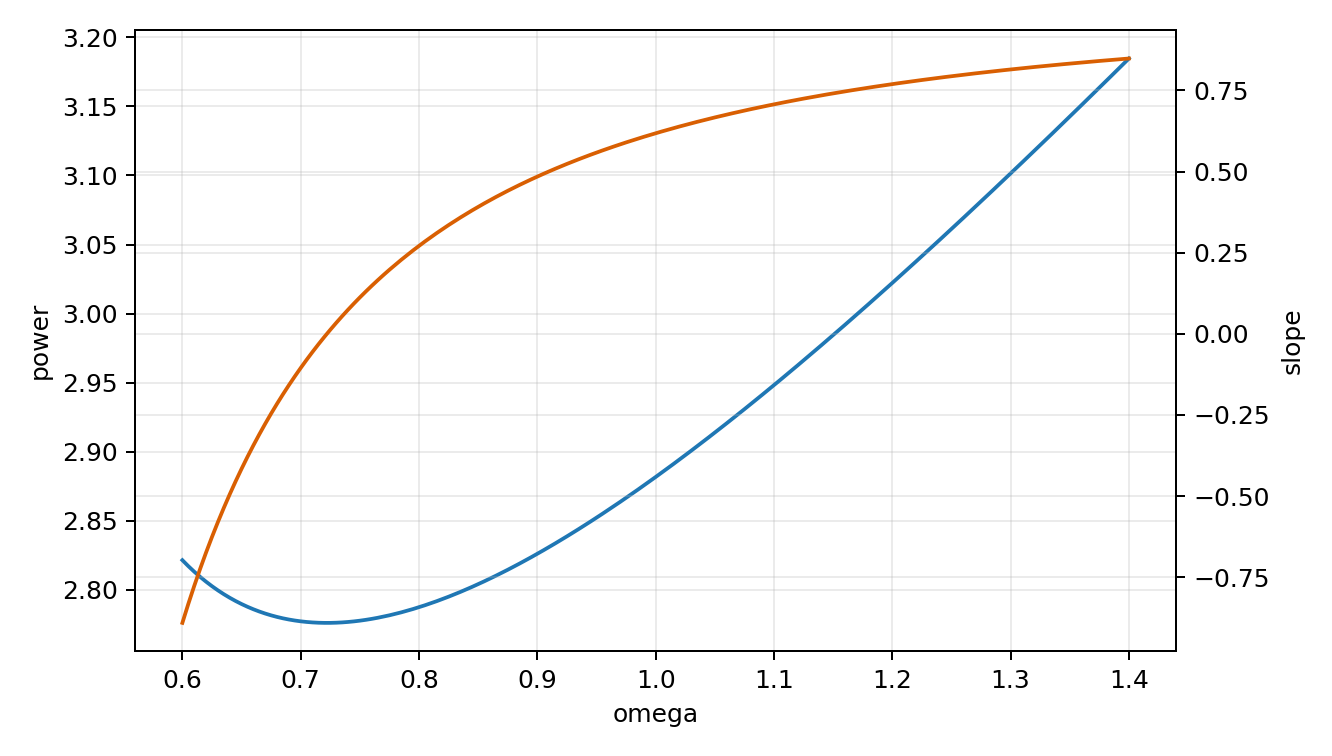
\includegraphics[width=0.77\textwidth]{FIN_Programs_507_516_Figures/p509_vk_slope.png}
\caption{Power and Vakhitov--Kolokolov slope. The sign change separates two conditional stability regimes.}
\end{figure}

\paragraph{Verdict.} Orbital stability at $\omega=1$ has strong finite-matrix support, but the eigenvalue and slope margins have not yet been enclosed by proof-grade intervals. The complete frequency tube cannot be labelled stable.

\section{P510 --- mobility test and its falsification}

The conventional Peierls--Nabarro comparison requires site- and bond-centred localized stationary states at equal conserved power. The P497 site state has
\[
 P_{\rm site}=2.88167720,\qquad \operatorname{IPR}=0.65457832.
\]
The same-frequency bond state has power $4.56985156$ and IPR $0.33540584$. Continuing it downward in $\omega$, its minimum power while still satisfying the declared localization threshold is
\[
 P_{\rm bond,min}^{\rm loc}=4.06764129>P_{\rm site}.
\]
It then joins the uniform branch. Hence no localized equal-power bond comparator exists for the P497 state and the proposed PN barrier is undefined.

\begin{figure}[H]
\centering
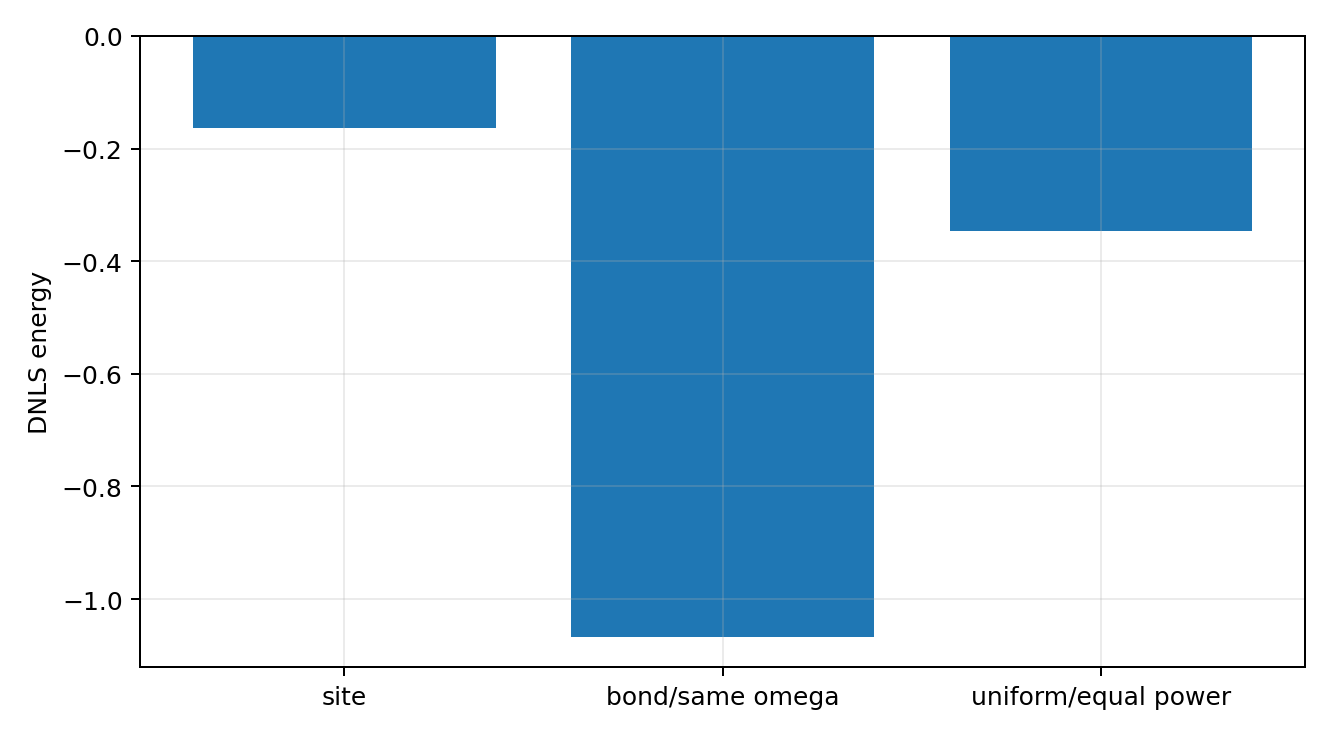
\includegraphics[width=0.74\textwidth]{FIN_Programs_507_516_Figures/p510_pn_barrier.png}
\caption{Energies of states that are not all comparable at fixed power. The plot documents why a conventional PN number cannot be reported honestly.}
\end{figure}

The twelve translated site states have equal energy to $1.34\times10^{-15}$, but degeneracy does not supply a continuous translation coordinate or motion. P510 therefore refutes one proposed mobility test rather than proving pinning or travel.

\section{P511 --- localization under positive spectral memory}

Let the positive P490 Stieltjes response be
\[
 \sigma(z)=\sum_j\frac{r_j}{z+c_j},\qquad r_j,c_j>0.
\]
The stable hidden relaxation realization motivates the row-sum-zero Bernstein loading
\[
 M=\sigma(0)I-\sum_j r_j(A+c_jI)^{-1}\succeq0,
 \qquad M\mathbf1=0.
\]
Numerically, $\operatorname{spec}M\subset[-7\times10^{-17},0.18820975]$ and the row-sum residual is $1.17\times10^{-16}$. Replacing $A$ by $A+\varepsilon M$ and continuing $0\le\varepsilon\le1$ yields at full loading
\[
 \operatorname{IPR}=0.62080181,\qquad
 \text{peak fraction}=0.78252530,
 \qquad \|F\|_\infty=4.44\times10^{-16}.
\]

\begin{figure}[H]
\centering
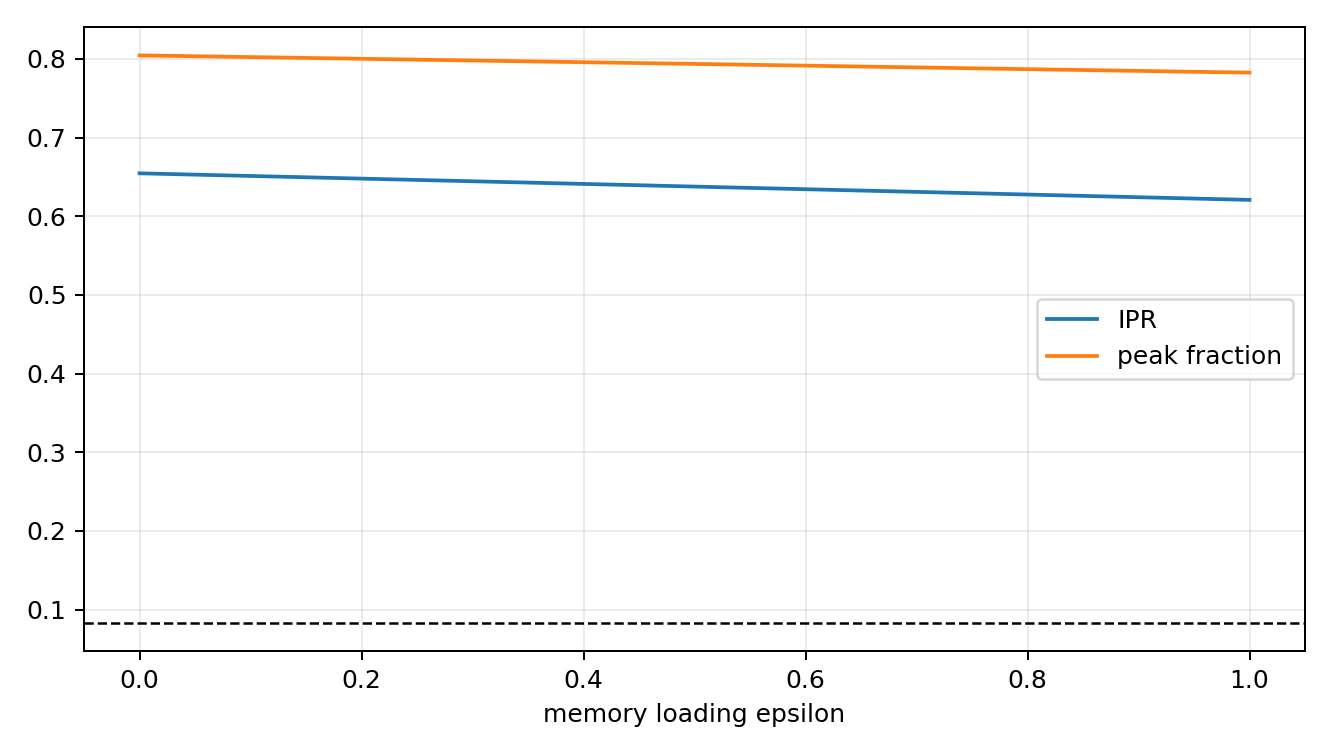
\includegraphics[width=0.77\textwidth]{FIN_Programs_507_516_Figures/p511_memory_localization.png}
\caption{The stationary localized branch remains far from the delocalized IPR $1/12$ throughout the declared memory loading.}
\end{figure}

This is stationary zero-frequency robustness, not a theorem for the full hidden temporal dynamics, non-Markovian stability, or an internally derived environment.

\section{P512 --- a transcendental strict frequency ratio}

The strict decimal phases have the exact rational forms
\[
 \phi=\frac{650}{4000},\qquad \omega=\frac{743}{4000},\qquad
 \phi+d\omega=\frac{650+743d}{4000}.
\]
Put $z=e^{i/4000}$. Since $i/4000$ is a nonzero algebraic number, the Lindemann--Weierstrass theorem implies that $z$ is transcendental. Moreover,
\[
 \cos(\phi+d\omega)=\frac{z^{650+743d}+z^{-(650+743d)}}{2}.
\]
All remaining Fourier coefficients are algebraic: $d^{9/5}$ is algebraic and the $12$th-root-of-unity Fourier factors are algebraic. Therefore every strict eigenvalue $\lambda_m$ is a Laurent polynomial $P_m(z)$ with algebraic coefficients.

\begin{theorem}[Strict two-frequency irrationality]
The ratio $\lambda_2/\lambda_1$ is transcendental, hence irrational.
\end{theorem}
\begin{proof}
For $m=1$, the cyclic distance-six coefficient is proportional to $1-(-1)^1=2$, so $P_1$ has a nonzero highest term $z^{5108}$. For $m=2$, the same coefficient is $1-(-1)^2=0$, and all remaining phase exponents are at most $4365$. Thus $P_1$ and $P_2$ are not proportional. If $P_2(z)/P_1(z)=a$ were algebraic, then the nonzero Laurent polynomial $P_2-aP_1$ would vanish at $z$. After clearing negative powers, $z$ would satisfy a nonzero polynomial with algebraic coefficients and would be algebraic, a contradiction. Finally, $P_1(z)=\lambda_1>0$ because all strict weights are positive and mode one is nonconstant.
\end{proof}

This closes the open arithmetic part of P499. The two-frequency phase map is injective and nonperiodic. It still carries no absolute unit and supplies no preferred clock origin.

\section{P513 --- a conservative convergence-rate certificate}

The even/odd attenuation symbols belong to the Wiener algebra because $h_d=(1+d^{9/5})^{-1}\in\ell^1$. Splitting at a finite cutoff, bounding the tail by
\[
 2\sum_{d>M}h_d\le\frac{2}{9/5-1}M^{1-9/5},
\]
and applying the resolvent identity yields an absolute response-error envelope. A truncated-symbol derivative bound pays the trapezoidal quadrature error. The combined asymptotic rate is
\[
 O(n^{-(9/5-1)})=O(n^{-0.8}).
\]

The conservative normalization denominator is not positive for $C_{384}$ or $C_{768}$. It first becomes positive at $C_{1536}$; the maximum normalized bounds are $27.14$, $4.77$ and $1.85$ at $C_{1536},C_{3072},C_{6144}$, respectively, whereas observed errors are near $10^{-3}$--$10^{-4}$.

\begin{figure}[H]
\centering
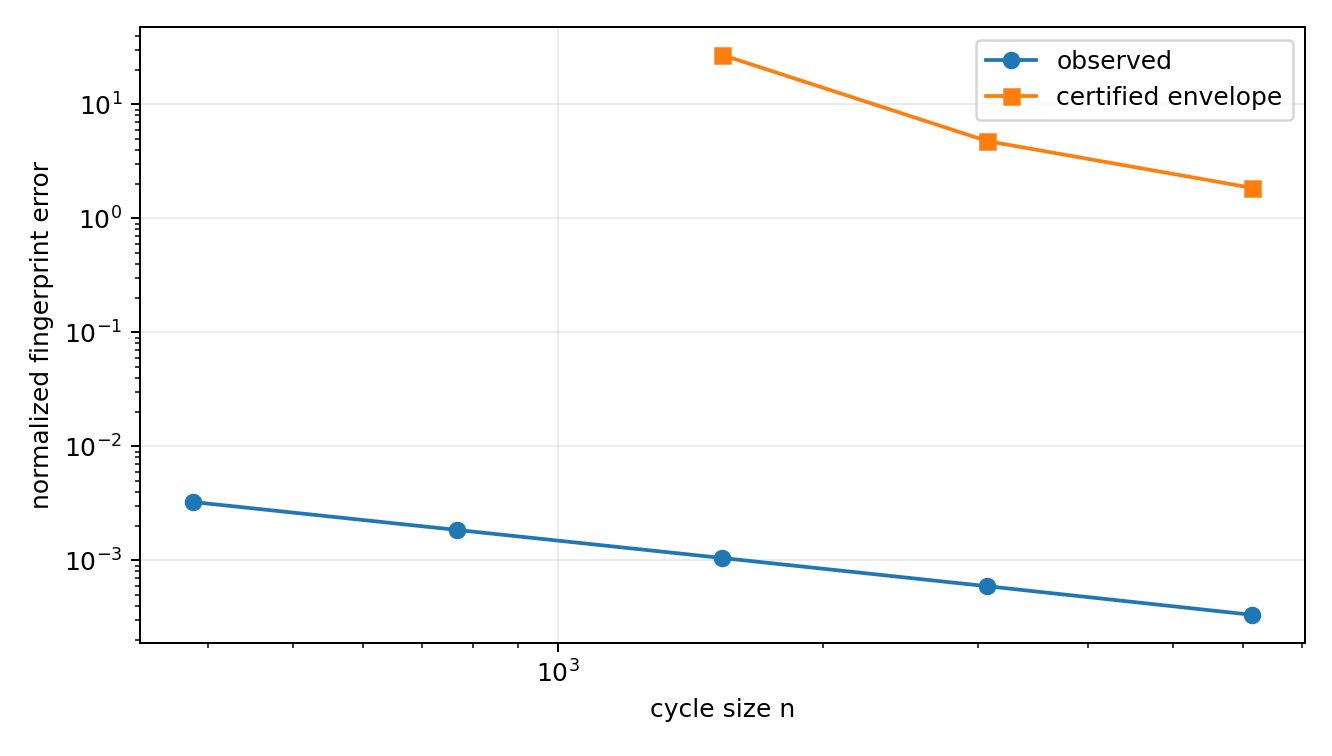
\includegraphics[width=0.77\textwidth]{FIN_Programs_507_516_Figures/p513_context_bound.png}
\caption{Observed error versus the proof-oriented Wiener--resolvent envelope. The large gap is reported, not hidden.}
\end{figure}

P513 certifies the rate class but refutes the hope that this elementary norm argument will sharply certify the P501 $C_{384}$ value.

\section{P514 --- the global PSD phase diagram}

All eleven nonconstant Fourier eigenvalues of the Legacy*--strict homotopy were evaluated outward on an adaptive partition of the complete unit interval. Five hundred and twelve initial boxes refined to 573 terminal boxes. The result is
\begin{align*}
 0\le t\le0.7008185567101464 &\quad\Longrightarrow\quad L(t)\not\succeq0,\\
 0.7008185570593923\le t\le1 &\quad\Longrightarrow\quad L(t)\succeq0.
\end{align*}
The only unresolved interval is
\[
 [0.7008185567101464,\ 0.7008185570593923],
\]
of width $3.49246\times10^{-10}$. It contains the P502 root. There are no hidden earlier PSD windows. This is a global interval classification, not merely a sign check at two endpoints.

The result does not make the interpolated path canonical or source the strict endpoint.

\section{P515 --- robust one-context synthetic separation}

The P504 context is retained:
\[
 t=0.55,\qquad \text{Fourier-1 preparation},\qquad \text{Fourier measurement}.
\]
Declare the hypothetical budgets
\[
 D_{\rm prep}\le0.005,\qquad
 D_{\rm POVM}\le0.005,\qquad
 |\delta t|\le0.002.
\]
CPTP or stochastic contraction pays preparation error. Measurement error is paid directly in total variation. Uniform generator-norm speed bounds pay timing error. For each model pair,
\[
 D_{\rm TV}^{\rm actual}\ge D_{\rm TV}^{\rm nominal}
 -2(0.005+0.005)-(v_i+v_j)0.002.
\]
All six lower bounds remain positive. The minimum, for dephasing versus revival, is
\[
 D_{\rm TV}^{\rm robust}\ge0.2024144925.
\]
This is a conditional robustness theorem for explicit numerical budgets, not evidence that a physical instrument meets them.

\section{P516 --- when a parameter law becomes identifiable}

P506 proves that no finite record identifies an unrestricted continuous trajectory. P516 adds a finite-dimensional law class:
\[
 \dot p(t)=\sum_{k=0}^{r}c_kt^k,\qquad p(0)=p_{\rm legacy},\qquad r=0,1,2,
\]
without inserting the strict endpoint. There are $5(r+1)$ unknown scalar coefficients.

\begin{theorem}[Conditional dimension-minimal design]
Fewer than $5(r+1)$ scalar observations cannot locally identify the degree-$r$ law. The reported five-distance observations at $r+1$ distinct nonzero times attain rank $5(r+1)$ and therefore meet this lower bound.
\end{theorem}
\begin{proof}
The observation derivative has at most as many rows as scalar observations, so fewer than the parameter dimension cannot have full column rank. For the reported designs the computed square sensitivity matrices have nonzero smallest singular values.
\end{proof}

The best audited designs all use distances $\{0,1,3,4,6\}$. Their condition numbers grow rapidly:
\[
 \kappa_0=985,\qquad \kappa_1=1.21\times10^4,\qquad
 \kappa_2=1.01\times10^5.
\]
Thus a law can become locally identifiable only after its finite model class is supplied, and higher-order laws rapidly become fragile. This does not evade P506's unrestricted no-go.

\section{Integrated interpretation}

\subsection{What is now theorem-level}

\begin{enumerate}
\item The current strict quadratic core does not select the nonlinear cubic sign or coefficient.
\item Conditional on focusing DNLS, one unique localized real stationary branch exists without folds for the complete strict-coupling interval.
\item The ratio of the first two nonzero strict frequencies is transcendental and the two-frequency clock is injective and nonperiodic.
\item The Legacy*--strict homotopy is globally non-PSD below one narrow transition bracket and PSD above it.
\item Within the stated finite law classes, dimension-minimal observation counts are known.
\end{enumerate}

\subsection{What remains conditional or refuted}

\begin{itemize}
\item Orbital stability at $\omega=1$ has strong GSS/VK evidence but no interval eigenvalue certificate.
\item The conventional equal-power PN mobility test is unavailable for the P497 power because no localized bond comparator exists.
\item Memory robustness concerns a supplied stationary Bernstein loading, not a derived temporal environment.
\item The elementary Wiener bound is far too loose to certify the observed $C_{384}$ normalized error.
\item The robust tester and polynomial law designs depend on hypothetical budgets and model classes.
\item No result generates an absolute time, length, action, mass or energy unit.
\end{itemize}

\claimbox{\textbf{Updated interpretation.} The strict operator is a certified localization-capable generator once a focusing fourth-order variational jet is supplied. The missing physical principle has moved one mathematical level upward: it must choose the nonlinear jet, its sign and scale. Quadratic spectral information alone provably cannot do so.}

\section{Recommended next bounded studies P517--P526}

\begin{longtable}{@{}p{0.09\textwidth}p{0.29\textwidth}p{0.45\textwidth}p{0.09\textwidth}@{}}
\caption{Next analytical and small-compute programmes.}\\
\toprule
Program & Objective & Acceptance criterion & Priority\\
\midrule
\endfirsthead
\toprule
Program & Objective & Acceptance criterion & Priority\\
\midrule
\endhead
P517 & Information-functional fourth-order jet & Audit entropy, Fisher, compression and admissible local actions for a uniquely signed quartic variation; otherwise prove family-level sign freedom. & 10/10\\
P518 & Independent exact replay of O212 & Rationalize the Krawczyk matrices and export a dependency-minimal checker reproducing all 801 inclusions. & 9/10\\
P519 & Interval orbital-stability theorem & Enclose $L_-$, $L_+$ and $dP/d\omega$ on a neighbourhood of $\omega=1$ and isolate the VK turning point. & 10/10\\
P520 & Bond-branch bifurcation and mobility alternatives & Locate the bond-to-uniform transition, folds and phase-kicked moving breathers without reporting an undefined PN barrier. & 8/10\\
P521 & Full temporal memory stability & Introduce explicit hidden relaxation variables and prove or refute persistence and stability of the localized state in the augmented flow. & 9/10\\
P522 & Multi-frequency clock and scale no-go & Extend the transcendence argument to a maximal rationally independent frequency set and restate the absolute-scale obstruction. & 8/10\\
P523 & Fractional-Hölder context bound & Replace the loose derivative/Wiener estimate by a sharp $C^{0,0.8}$ quadrature and resolvent bound targeting $C_{384}$. & 8/10\\
P524 & Portable exact PSD checker & Export all P514 interval boxes and a standard-library replay with independent sign verification. & 7/10\\
P525 & Detector-level robustness model & Add loss, dark counts, coarse graining and configuration drift to O219 and determine the admissible error polytope. & 9/10\\
P526 & Law-class selection/no-free-lunch audit & Compare competing low-dimensional parameter laws with frozen synthetic hold-out data and prove what remains prior-dependent. & 9/10\\
\bottomrule
\end{longtable}

P517 is the conceptual priority: it tests whether the new quartic obligation can emerge from FIN's information language. P519 is the strongest immediate proof upgrade. P521 determines whether the stationary memory result survives as actual dynamics.

\section{Reproducibility}

Primary artifacts:
\begin{itemize}
\item \path{fin_programs_507_516_research.py};
\item \path{test_fin_programs_507_516.py};
\item \path{FIN_Programs_507_516_Results.json};
\item \path{FIN_Programs_507_516_Summary.csv};
\item \path{FIN_Programs_507_516_Figures/}.
\end{itemize}

Replay commands:
\begin{verbatim}
MPLCONFIGDIR=/tmp/fin-mpl-1051 \
  python3 fin_programs_507_516_research.py
MPLCONFIGDIR=/tmp/fin-mpl-1051 \
  python3 -m unittest -v test_fin_programs_507_516.py
pdflatex -interaction=nonstopmode -halt-on-error \
  FIN_Programs_507_516_Nonlinear_Source_and_Certified_Localization_Report_EN.tex
\end{verbatim}

The complete batch uses 12-variable stationary solves, interval matrices of order 12, 401 parametric charts, 400 interface checks, 573 PSD boxes, FFT arrays of length at most 262144, and finite synthetic probability tables. It is designed for an ordinary local workstation.

\section{Final verdict and nonclaims}

P507--P516 materially improve the mathematical status of the FIN localization programme. Conditional on the focusing DNLS law, the localized branch is now a complete interval-certified object rather than a floating continuation. Its principal two-frequency clock has a theorem-level transcendental ratio. Its stationary localization is robust against one explicit positive spectral-memory loading. The Legacy*--strict homotopy has a global PSD phase classification.

The same batch proves the central limitation. The strict quadratic core cannot choose the nonlinear fourth-order jet. Consequently, the certified localized branch does not yet emerge from FIN alone. The missing object is now sharply typed: a nonlinear source functional or axiom that fixes sign, strength and ultimately dimensional scale.

No result here discharges $QW$-2191, selects orientation, creates physical units, completes the Legacy*--strict source bridge, transfers a legacy physical role, supplies laboratory evidence, derives particles, Standard Model, gravity or $L_{\rm total}$, or closes a Theory of Everything.

\end{document}
